\documentclass[12pt,addpoints]{exam}
\usepackage[utf8]{inputenc}
\usepackage[T1]{fontenc}
\usepackage[brazil]{babel}
\usepackage[a4paper, margin=2cm]{geometry}
\usepackage{graphicx, amsmath, amsfonts, amssymb, xcolor, url, tikz, pgfplots, subfigure}

\newcommand{\disciplina}{Laboratório de Princípios de Comunicações}
\newcommand{\periodo}{2020.1}
\newcommand{\avaliacao}{Guia de Experimentos 3}
\newcommand{\tema}{Modulação e Desmodulação em Amplitude}
%\newcommand{\professor}{Bruno\ B.\ Albert e Edmar C.\ Gurjão}
%\newcommand{\professor}{Leocarlos B.\ S.\ Lima e Edson P.\ da Silva}
\newcommand{\professor}{Edson P.\ da Silva e Luciana Veloso}
%\newcommand{\professor}{Edmar C.\ Gurjão e Luciana Veloso}
%\newcommand{\professor}{Bruno\ B.\ Albert e Edson P.\ da Silva}

\pagestyle{head}
\firstpageheader{}{}{}
\runningheader{Lab.\ Princ.\ Comunicações}{\avaliacao}{Página \thepage}
\runningheadrule
\pointpoints{ponto}{pontos}
\newcommand{\myscale}{0.4}
\newtheorem{exemplo}{Exemplo}[section]

\begin{document}
    
\noindent 
\includegraphics[height=2cm]{../Figuras/UFCGLogo.png} \hfill
\begin{minipage}{.66\textwidth} \large \centering \vspace{-1.8cm}
    Universidade Federal de Campina Grande -- UFCG \\
    Unidade Acadêmica de Engenharia Elétrica -- UAEE \\
    Curso de Graduação em Engenharia Elétrica
\end{minipage}
\hfill 
\includegraphics[height=2cm]{../Figuras/DEELogo.png} \\[12pt]

\noindent
\begin{tabular*}{\textwidth}{l @{\extracolsep{\fill}} r @{\extracolsep{6pt}} l}
    \textbf{\disciplina} && \\
    Período \periodo && \\
    \textbf{\avaliacao} && \\
    Tema(s): \tema && \\
    Professor(es): \professor && \\
\end{tabular*}
\noindent\rule[2ex]{\textwidth}{2pt}
    
\section{Introdução}

O presente guia descreve atividades experimentais a serem realizadas na disciplina Laboratório de Princípios de Comunicações do curso de graduação em Engenharia Elétrica da Universidade Federal de Campina Grande -- UFCG.

Os experimentos propostos deverão ser realizados no Laboratório de Princípios de Comunicações -- LPC, localizado na Central de Laboratórios da Unidade Acadêmica de Engenharia Elétrica da UFCG, empregando:
\begin{itemize}
    \item Computador com software GNU Radio Companion -- GRC (\url{http://gnuradio.org/}) instalado;
    \item Módulo USRP (do inglês \textit{Universal Software Radio Peripheral}) para transmissão e recepção de sinais numa abordagem conhecida como Rádio Definido por Software -- RDS.
\end{itemize}

Na seção \ref{sect:Preparacao} deste guia, propõe-se um conjunto de atividades de preparação a serem desenvolvidas pelo aluno antes da aula em que serão realizadas as práticas experimentais. Sem a realização prévia destas atividades pelo aluno, as práticas experimentais propostas ficarão comprometidas, tanto no tempo necessário para sua realização quanto no aproveitamento pelo aluno. Por essa razão, \textbf{o aluno só poderá realizar os experimentos em laboratório se apresentar ao professor no início da aula os resultados da preparação proposta}. 

A aula terá duração de duas horas e o aluno deverá entregar ao seu término, por escrito, respostas às questões referentes aos experimentos realizados propostas na Folha de Respostas (parte final do guia).

\section{Objetivos}

As práticas experimentais aqui propostas têm por objetivos:
\begin{itemize}
    \item Simular e analisar a modulação em amplitude;
    \item Simular e analisar o desmodulador síncrono;
    \item Simular e analisar o desmodulador por detecção de envoltória;
    \item Investigar o conceito de um receptor super-heteródino.
\end{itemize}

\section{Preparação} \label{sect:Preparacao}

\subsection{Estudo}

Revise e pesquise sobre os conceitos:
\begin{itemize}
    \item AM-DSB-SC e AM-DSB;
    \item Efeitos da incoerência de fase e de frequência na desmodulação síncrona no AM-DSB-SC e AM-DSB;
    \item Misturador (\textit{mixer}) e receptor super-heteródino.
\end{itemize}

\subsection{Problemas}

Os problemas propostos a seguir dever ser obrigatoriamente resolvidos e apresentados por escrito ao professor antes do início das práticas de laboratório. Os resultados destes problemas serão necessários para a realização dos experimentos propostos. 

\begin{questions}
  \question Considere um tom modulante de frequência $f_{m} = 200$~Hz e uma portadora de frequência $f_{c} = 5$~kHz. Esboce os gráficos, no tempo e na frequência, do sinal modulante $m(t) = \cos{2\pi f_{m}t}$ e do sinal modulado $\varphi_{DSB}(t) = A\cos{2\pi f_{c}t} + m(t)\cos{2\pi f_{c}t}$ considerando índices de modulação $\mu = 0.5$, $1.0$, $2.0$ e $\infty$. %($A = 0$).
  \question Descreva um diagrama de blocos de um receptor síncrono (coerente) para $\varphi_{DSB}(t)$.
  \question Descreva um diagrama de blocos de um detector de envoltória para $\varphi_{DSB}(t)$.
  \question O AM comercial usa um receptor super-heteródino com detecção de envoltória. Nele, o sinal recebido é deslocado para uma frequência intermediária $f_{i} = 455$~kHz. Quais as frequências do oscilador local do misturador para $f_{c} = 1050$, $1160$ e $1310$~kHz?
\end{questions}

\section{Experimentos}

A seguir são descritas práticas experimentais a serem realizadas pelo aluno em aula de laboratório. 

\subsection{Experimento 1 -- Modulação em Amplitude}

O objetivo deste experimento é analisar as modulações em amplitude DSB e DSB-SC.

\begin{enumerate}
    \item Antes de iniciar as atividades com o GRC, crie uma pasta para guardar os arquivos de seus experimentos e copie nela os modelos de diagrama (arquivos .GRC) disponibilizados pelo professor para esta aula. \textbf{Não deixe de realizar isso, pois o computador deste laboratório não é para seu uso pessoal e os arquivos que você utilizará serão alterados por você durante o experimento};
    \item Execute o software GRC e abra o arquivo \textbf{Labo3-1.grc}. A Figura \ref{fig:GRC_3-1} ilustra o diagrama deste experimento. Ele consiste na simulação da equação 
\begin{equation} \label{eq:am}
    \varphi_{DSB}(t) = [A + m(t)]\cos{2\pi f_{c}t},
\end{equation}
em que $A$ e $f_c$ podem ser alterados por suas respectivas réguas deslizantes disponíveis acima dos gráficos durante a execução do diagrama;
    \begin{figure}[htb]
        \centering
        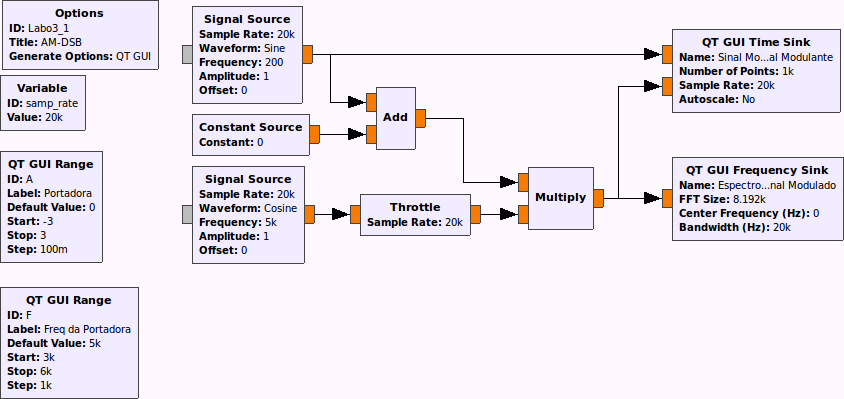
\includegraphics[scale=\myscale]{./Figuras/Labo3-1}
        \caption{Diagrama de blocos para análise da modulação em amplitude.} 
        \label{fig:GRC_3-1}
    \end{figure}
  \item Execute o diagrama e responda às questões propostas na Folha de Respostas.
\end{enumerate}

\subsection{Experimento 2 -- Desmodulação Síncrona}

O objetivo deste experimento é observar o efeito do desvio de fase e do desvio de frequência num receptor coerente.

\begin{enumerate}
    \item  Abra o arquivo \textbf{Labo3-2.grc} disponibilizado pelo professor. A Figura \ref{fig:GRC_3-1b} ilustra o diagrama deste experimento. Ele consiste do modulador visto no Experimento 1 e de um desmodulador síncrono (coerente), ou seja, o oscilador do receptor tem a mesma frequência e a mesma fase da portadora gerada no transmissor; 
    \begin{figure}[htb]
        \centering
        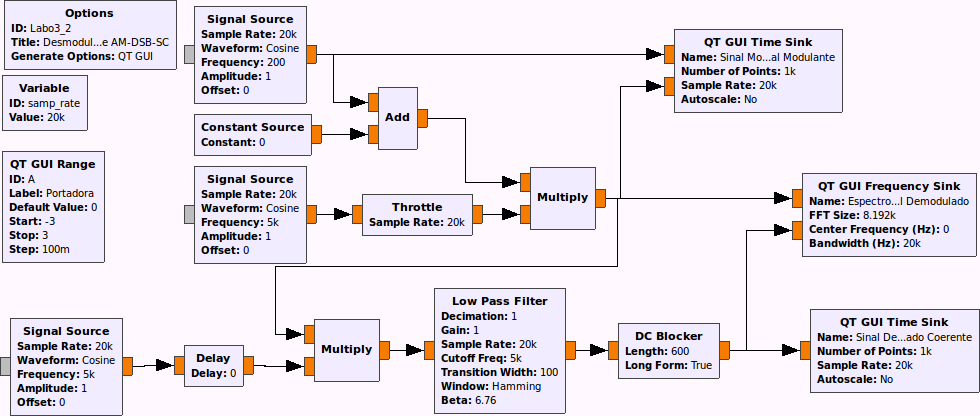
\includegraphics[scale=\myscale]{./Figuras/Labo3-2}
        \caption{Diagrama de blocos de um desmodulador síncrono.} 
        \label{fig:GRC_3-1b}
    \end{figure}
  \item Execute o experimento e observe que o sinal desmodulado tem metade da amplitude do sinal transmitido.
  % \item  Altere o índice de modulação e observe que a desmodulação coerente desmodula o sinal modulado para qualquer índice de modulação do transmissor.
  \item Responda as questões propostas na Folha de Respostas.
\end{enumerate}

\subsection{Experimento 3 -- Desmodulação por Detecção da Envoltória}

O objetivo deste experimento é observar o efeito da sobremodulação ($\mu > 1$) na desmodulação por deteção da envoltória (não coerente).

\begin{enumerate}
    \item  Abra o arquivo \textbf{Labo3-3.grc} disponibilizado pelo professor. A Figura \ref{fig:GRC_3-1c} ilustra o diagrama deste experimento. Ele consiste do modulador visto no Experimento 1 e de um desmodulador por detecção da envoltória (não coerente, ou seja, não existe um  oscilador local no receptor), bloco {\bf AM Demod};
    \begin{figure}[htb]
        \centering
        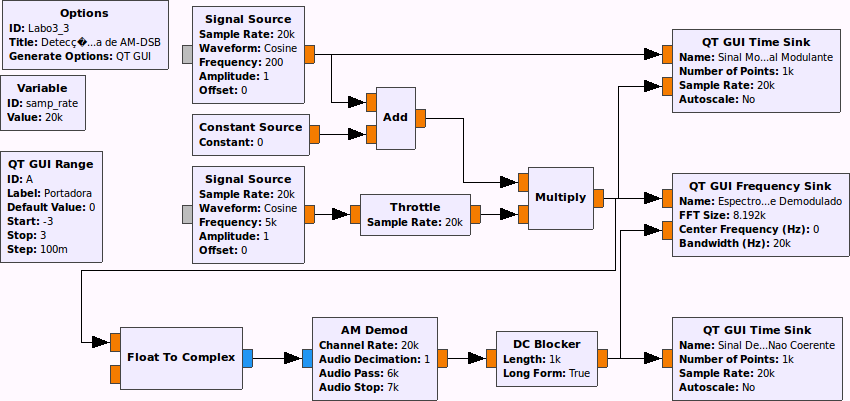
\includegraphics[scale=\myscale]{./Figuras/Labo3-3}
        \caption{Diagrama de blocos de um desmodulador por detecção da envoltória.} 
        \label{fig:GRC_3-1c}
    \end{figure}
  \item Responda as questões propostas na Folha de Respostas.
\end{enumerate}

\subsection{Experimento 4 -- Receptor Super-heteródino}

O objetivo deste experimento é mostrar o conceito de um receptor super-heteródino.

\begin{enumerate}
    \item  Abra o arquivo \textbf{Labo3-4.grc} disponibilizado pelo professor. A Figura \ref{fig:GRC_3-1d} ilustra o diagrama deste experimento. Ele consiste de um modulador AM-DSB para um sinal de voz gravado. No esquema, é possível alterar as frequências da portadora e de sintonia do receptor bem como a amplitude da portadora. A frequência intermediária é $fi = 25$~kHz, de modo que toda vez que uma frequência é sintonizada o sinal é transladado para $fi$. 
    \begin{figure}[htb]
        \centering
        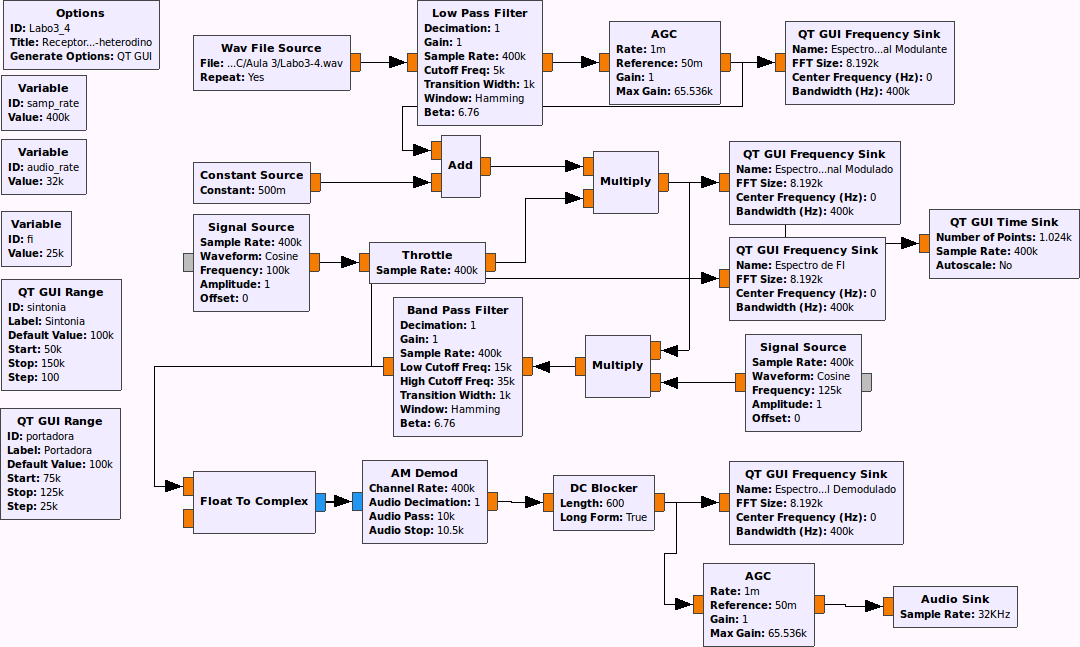
\includegraphics[scale=\myscale]{./Figuras/Labo3-4}
        \caption{Diagrama de blocos de um receptor super-heteródino.} 
        \label{fig:GRC_3-1d}
    \end{figure}
  \item Execute o experimento e responda as questões propostas na Folha de Respostas.
\end{enumerate}

\newpage \ \newpage \pagenumbering{arabic}

\noindent 
\includegraphics[height=2cm]{../Figuras/UFCGLogo} \hfill
\begin{minipage}{.66\textwidth} \large \centering \vspace{-1.8cm}
    Universidade Federal de Campina Grande -- UFCG \\
    Unidade Acadêmica de Engenharia Elétrica -- UAEE \\
    Curso de Graduação em Engenharia Elétrica
\end{minipage}
\hfill 
\includegraphics[height=2cm]{../Figuras/DEELogo} \\[12pt]

\noindent
\begin{tabular*}{\textwidth}{l @{\extracolsep{\fill}} r @{\extracolsep{6pt}} l}
    \textbf{\disciplina} && \\
    Período \periodo && \\
    \textbf{\avaliacao\ -- Folha de Respostas} && \\
    Tema(s): \tema && \\
    Professor(es): \professor && \\[12pt]
    \textbf{Aluno:} \hrulefill & \textbf{Data:} \makebox[3cm]{\hrulefill} & \\
\end{tabular*}
\noindent\rule[2ex]{\textwidth}{2pt}

\section*{Experimento 1 -- Modulação em Amplitude}

\begin{questions}
    \question Para $A = 0$ temos um transmissor AM-DSB-SC, esboce o gráfico no domínio da frequência obtido e identifique as bandas laterais do sinal modulado. Apresente todos os valores pertinentes com suas unidades no gráfico. Qual o índice de modulação nesse caso?
    \makeemptybox{5cm}
    
    \question Faça $A = 1$ (deslizando a respectiva régua) observe no espectro de frequência a introdução do espectro da portadora  em relação a questão anterior, quando $A=0$. Qual o novo índice de modulação? Qual a potência média da portadora? Qual a amplitude da portadora em dB no espectro de frequência?
    \fillwithlines{0.25in}
    
    \question Faça $A = 3$ observe o espectro de frequência. Qual o novo índice de modulação? Qual a potência média da portadora? Qual a amplitude da portadora em dB no espectro de frequência?
    \fillwithlines{0.25in}
    
    \question Qual o esquema mais eficiente em termos de potência do transmissor, $A = 1$ ou $A = 3$? Justifique.
    \fillwithlines{0.75in}
    
    \question Altere a frequência da portadora deslizando a sua respectiva régua. O que aconteceu com o sinal modulado? (Observe o gráfico em frequência.)
    \fillwithlines{0.5in}
    
%    \question \textbf{Exp.\ 1} $\Rightarrow$ Coloque uma onda quadrada como mensagem e ajuste o parâmetro \textbf{Offset} para $-0.5$. Execute experimento para $A = 0$ e verifique que não há mais diferenças nas amplitudes do sinal. Explique onde está a diferença entre os níveis da onda quadrada? Esse fato não ocorre para $A \ne 0$. Observe também o que ocorreu com o espectro do sinal modulado.
%    \fillwithlines{1in}
    
    % \question \textbf{Exp.\ 2} $\Rightarrow$ Por que são necessários o filtro passa-baixas e o bloqueador DC no desmodulador? Como sugestão, retire-os um de cada vez e observe o que ocorre.
    % \fillwithlines{1in}
\end{questions}

\section*{Experimento 2 -- Desmodulação Síncrona}

\begin{questions}
    \question Altere o índice de modulação deslizando a régua da amplitude da portadora e observe que a desmodulação coerente desmodula o sinal modulado para qualquer valor do índice de modulação do transmissor. Por que?
    \fillwithlines{0.5in}

    \question Retire o filtro passa-baixas e explique sua utilidade observando o gráfico em frequência.
    \fillwithlines{0.5in}
    
    \question Retorne o filtro ({\bf Ctrl-Z}). A fase do oscilador local no receptor pode ser alterada pelo bloco \textbf{Delay} que atrasa o sinal num tempo correspondente a um certo número de amostras. Qual é esse tempo para um atraso de uma amostra? Assim, cada amostra corresponde a um atraso de $1/f_{s} = 1/25000 =  40$~$\mu$s, em que $f_{s}$ é a frequência de amostragem, ou a uma defasagem de $\frac{1/f_{m}}{1/f_{s}}.360º = \frac{1/5000}{1/25000}.360º = 72º$ no oscilador local. Faça esse atraso igual a 1 amostra. Houve distorção no sinal desmodulado em relação ao sinal mensagem? Explique.
    \fillwithlines{0.75in}
    
    \question Retorne o atraso para 0 amostras. Altere o oscilador local do receptor para 5050~Hz e execute o experimento. Por que o sinal desmodulado está distorcido em relação ao sinal mensagem? Seria aceitável 1~Hz de diferença (oscilador local em 5001~Hz)?
    \fillwithlines{0.75in}
\end{questions}

\section*{Experimento 3 -- Desmodulação por Detecção da Envoltória}

\begin{questions}
    \question Para amplitudes da portadora em 0.0, 0.5, 1.0 e 2.0 (use  a régua deslizante para isso), observe os resultados (sinais desmodulados) no tempo e na frequência para cada valor. Quais resultados correspondem ao sinal modulante (mensagem)? Por que?
    \fillwithlines{0.75in}
\end{questions}

\section*{Experimento 4 -- Receptor Super-heteródino}

\begin{questions}
    \question Por que o sinal sintonizado é sempre transladado para $f_{i} = 25$~kHz? Observe o bloco \textbf{Signal Source} correspondente ao oscilador local do receptor e use os resultados da preparação.
    \fillwithlines{1in}
    
    \question Na prática é possível se determinar o índice de modulação pela observação da envoltória do sinal modulado. Considere $S_{max}$ e $S_{min}$ os valores máximo e mínimo da envoltória respectivamente, então
    \begin{equation}
      \label{eq:mu100}
      \mu \times 100\% = \frac{S_{max} - S_{min}}{S_{max} + S_{min}}
      \times 100\%
    \end{equation}
    Calcule o índice de modulação do sinal de voz modulado desse experimento. Para qual valor de amplitude teríamos um indice de modulação de aproximadamente 1? Altere o índice de modulaçao para infinito ($A = 0$) e observe o que ocorre.
    \fillwithlines{0.5in}

%    \question Coloque o transmissor AM (a frequência da  portadora do transmissor) na frequência de 125~kHz. Sintonize na nova frequência, perceba que não precisa termos a frequência exata para que o sinal de voz seja capturado. Existe uma outra frequência de sintonia no receptor, além da de 125~kHz, em que o sinal é também desmodulado. A rádio em 125~kHz é uma rádio fantasma para essa frequência. Qual é essa frequência e por que isso ocorre?
%    \fillwithlines{1in}
\end{questions}

\end{document}
